\section{Conda ecosystem}
\subsection{a case of bioconda}

\begin{frame}{Conda system}
\begin{itemize}
\item<1-3> \hyperlink{https://www.anaconda.com/}{Anaconda}
	\begin{itemize}
	\item Open source distribution
    \item Cross platform
    \item Available on cluster without admin whrite
    \item Thousands of available tool in informatic and bioinformatic
	\end{itemize}
\item<2-3> \hyperlink{https://docs.conda.io/en/latest/miniconda.html}{Miniconda}
	\begin{itemize}
	\item A lightheight Anaconda version with minimal requirment
	\item Same advantages ad Anaconda
	\end{itemize}
\item<3> \hyperlink{https://docs.conda.io/projects/conda/en/latest/index.html}{Conda} 
\includegraphics[width=0.1\textwidth]{images/conda_logo.pdf} 
	\begin{itemize}[<4->]
	\item Package manager AND environment manager
	\item installed with Ana or Miniconda
	\item Python based but can also install tools from R, C++ or Julia...
	\end{itemize}
\end{itemize}
\end{frame}

\begin{frame}{Conda system}
\centering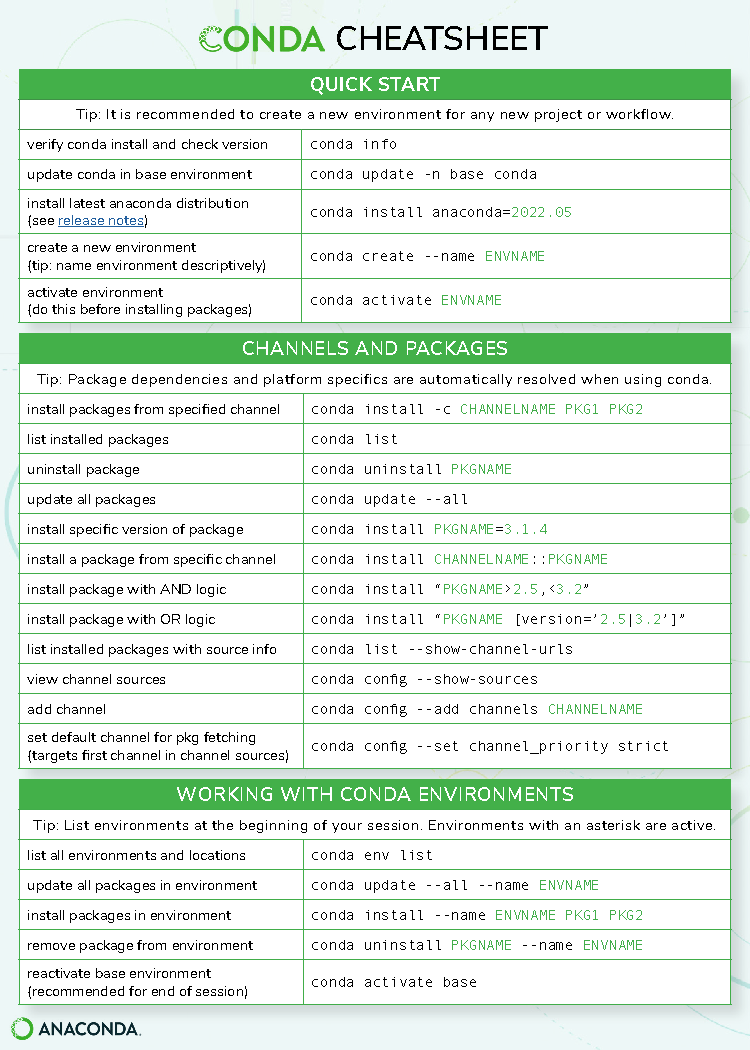
\includegraphics[width=0.45\textwidth]{images/conda_sheet_4.12.pdf}
\end{frame}
\begin{frame}{The channels and the tools}
The tools are packaged and available on several \textbf{channels}
\begin{minipage}[t]{0.48\linewidth}
\begin{itemize}[<2->]
\item Conda-forge
\item Anaconda
\end{itemize}
\end{minipage}
\begin{minipage}[t]{0.48\linewidth}
\begin{itemize}[<2->]
\item R
\item Bioconda --> Most of the bioinformatic tools
\end{itemize}
\end{minipage}
\onslide<3->{\centering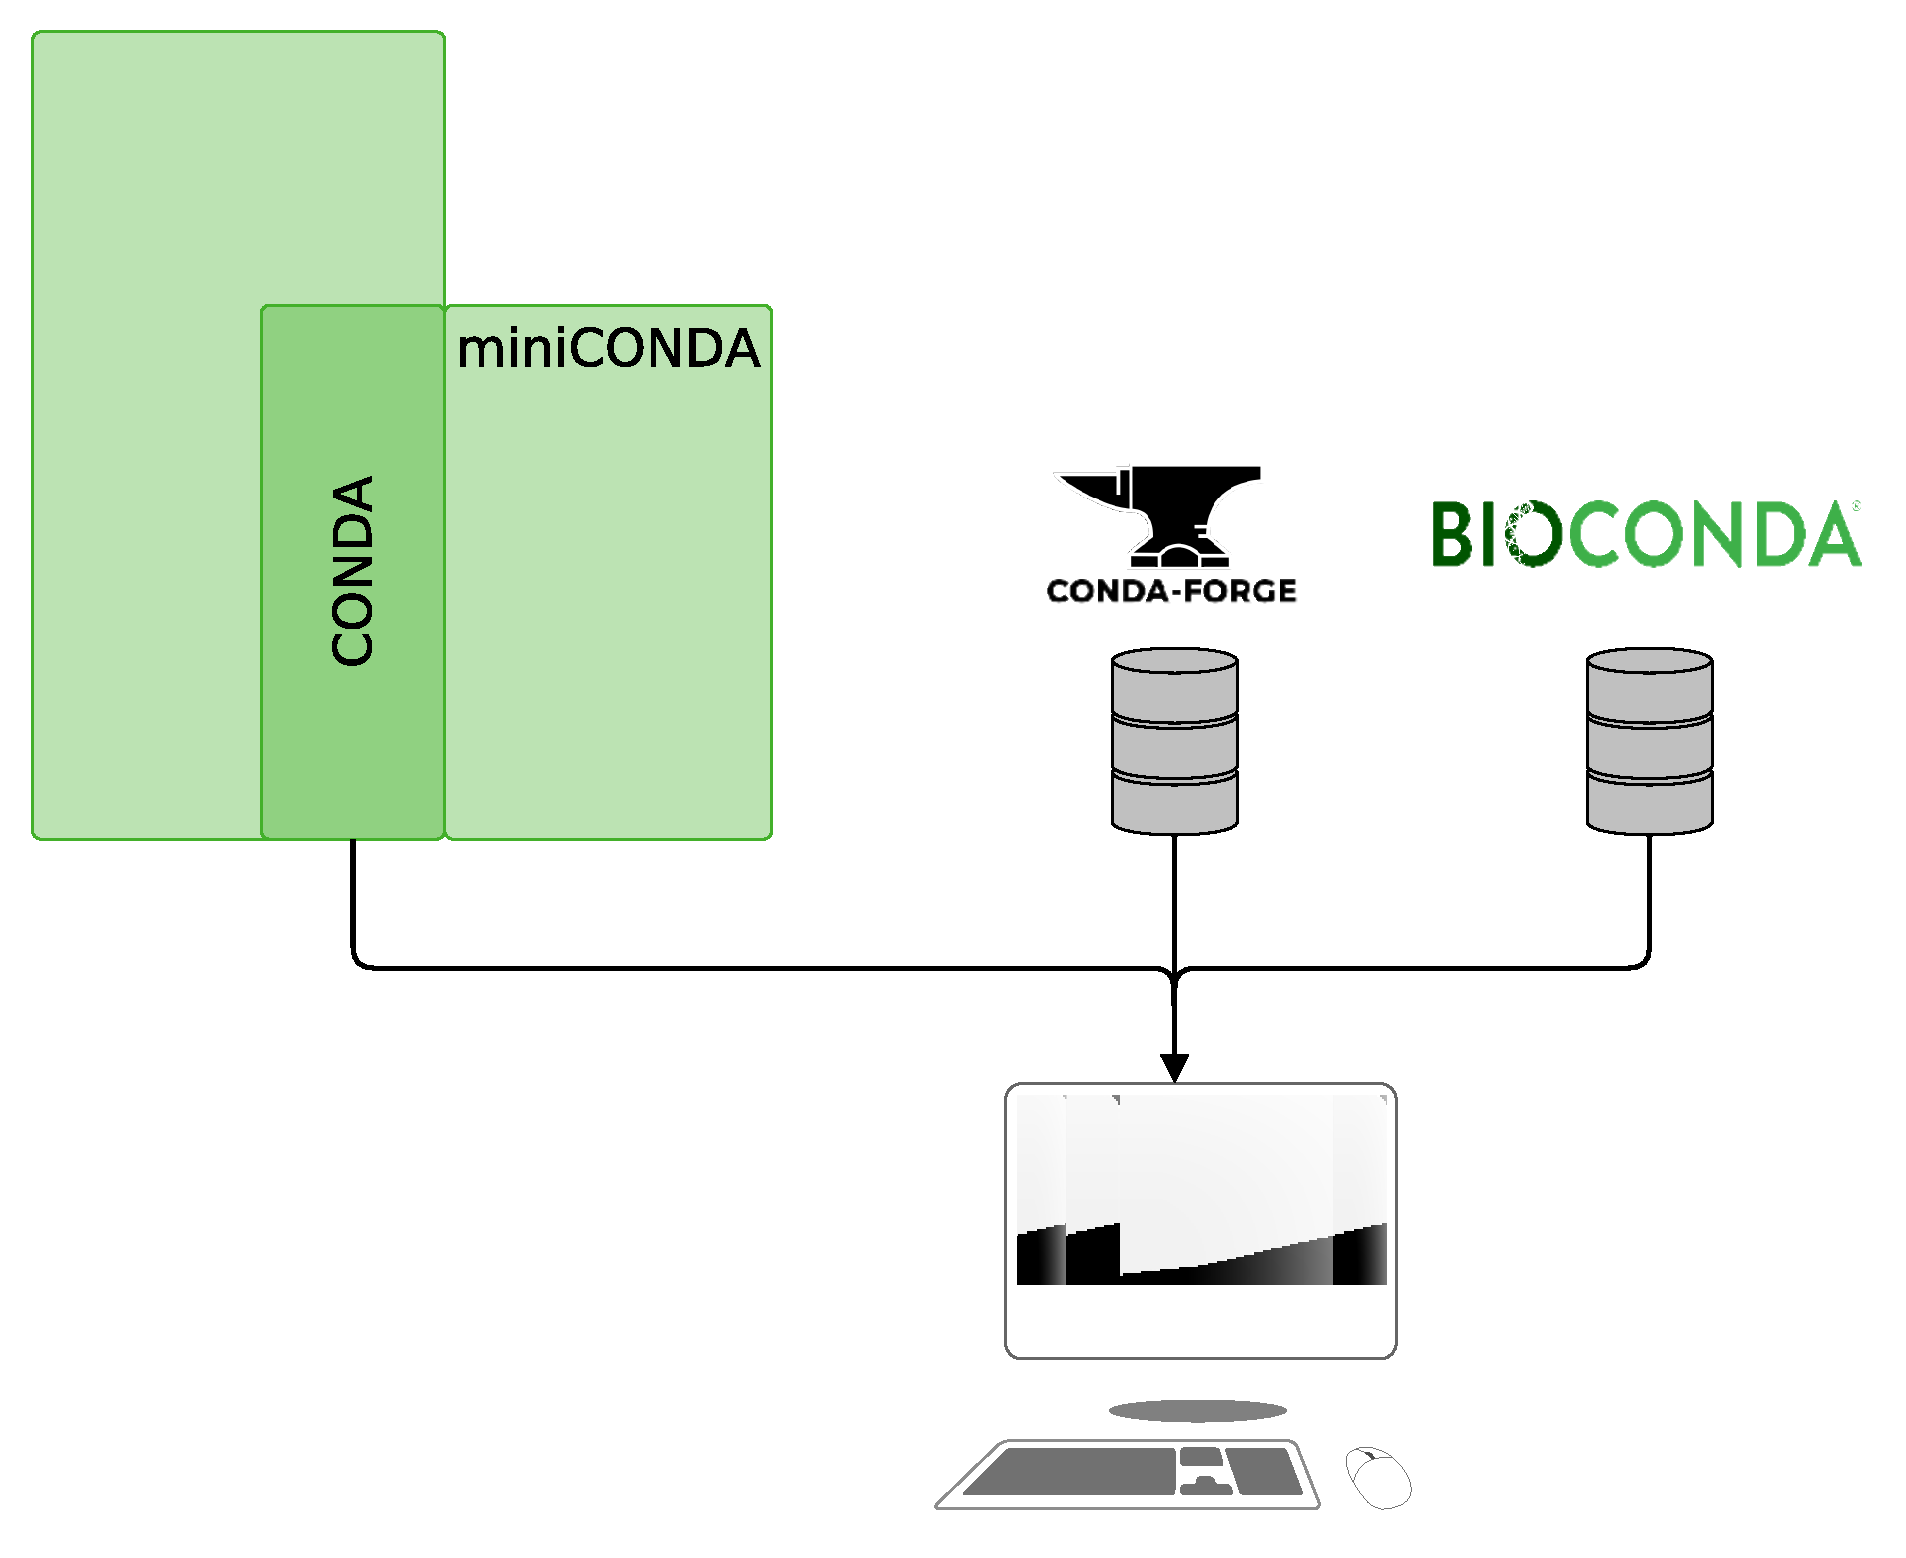
\includegraphics[width=0.5\textwidth]{images/conda_env_detail.pdf}\blfootnote{Bioconda: sustainable and comprehensive software distribution for the life sciences \textit{Grüning et al.}, Nature methods, 2018. DOI 10.1038/s41592-018-0046-7}}
\end{frame}

\begin{frame}{Basic commands}
\begin{columns}
\column{.48\textwidth}
\onslide<1->{
\begin{block}{Create environment}
\begin{itemize}
\item[\$] conda create -n [env\_name]
\item[\$] conda activate [env\_name]
\item[\$] conda deactivate [env\_name]
\end{itemize}
\end{block}}
\onslide<2->{
\begin{block}{list environment or packages}
\begin{itemize}
\item[\$] conda env list
\item[\$] conda list
\end{itemize}
\end{block}}
\column{.48\textwidth}
\onslide<3->{
\begin{block}{Search tools}
\begin{itemize}
\item[\$] conda search bowtie2
\item[\$] conda search -c bioconda bowtie2
\end{itemize}
\end{block}}
\onslide<4->{
\begin{block}{Install tools}
\begin{itemize}
\item[\$] conda install bowtie2
\item[\$] conda install -c bioconda bowtie2
\item[\$] conda install -c bioconda bowtie2=2.4.5
\end{itemize}
\end{block}}
\onslide<5->{
\begin{block}{Remove tools}
\begin{itemize}
\item[\$] conda remove bowtie2
\end{itemize}
\end{block}}
\end{columns}
\end{frame}

\begin{frame}{Environment resolution}
\only<1>{
Conda also manage environments to keep compatible
\begin{itemize}
\item Long time to solve environment resolution
\item Can fail and doesn't install
\end{itemize}}
\only<2>{\centering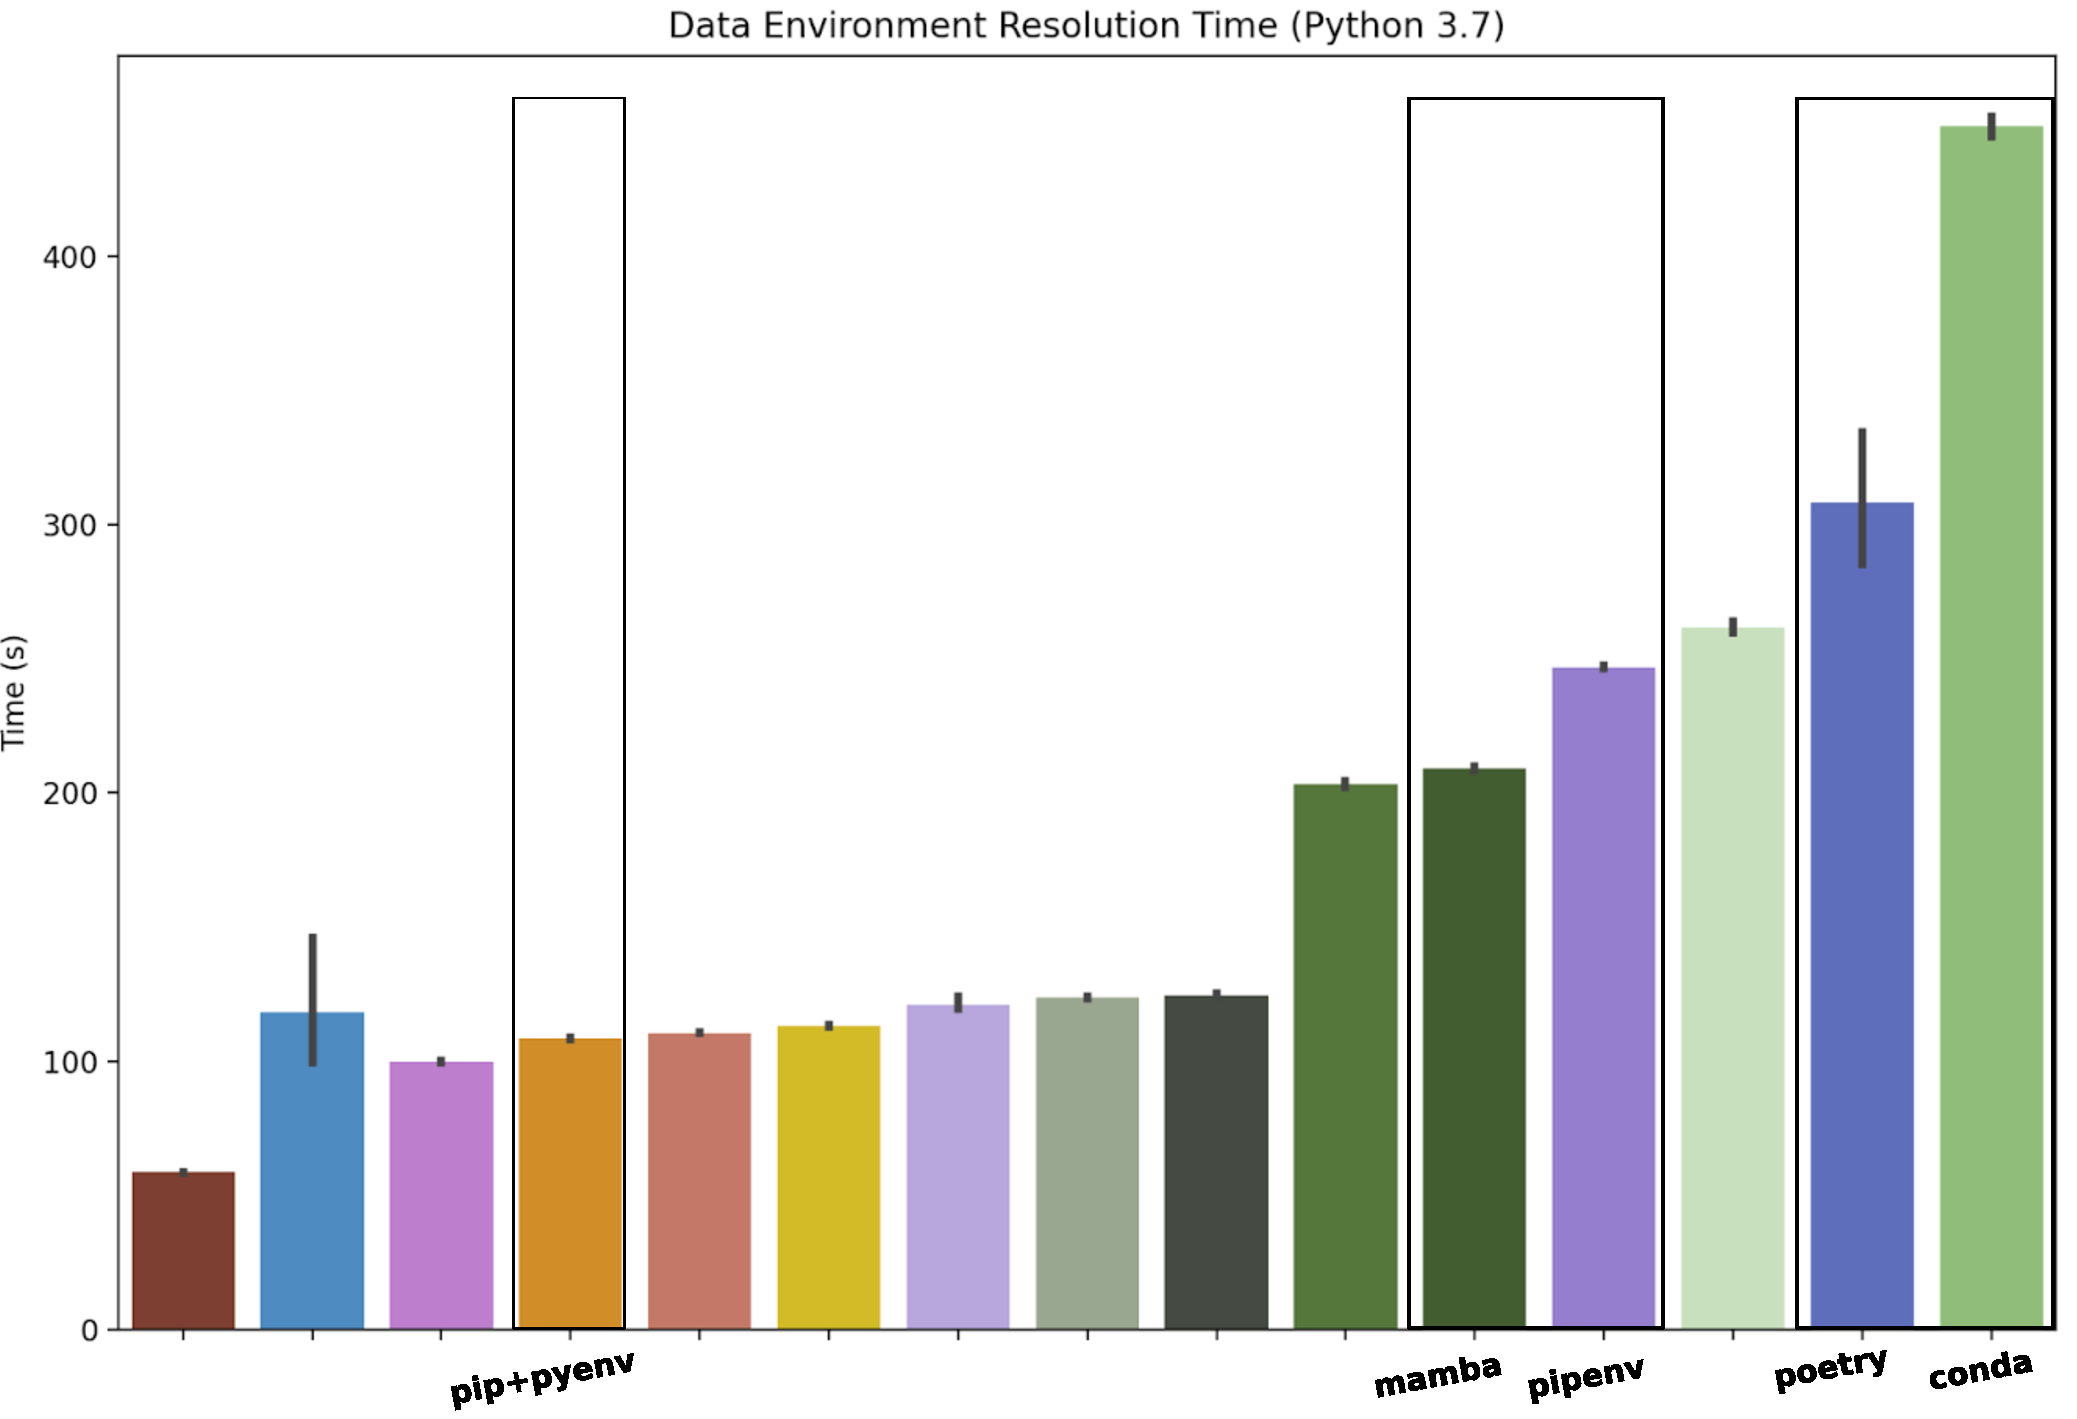
\includegraphics[width=0.7\textwidth]{images/conda_use.pdf}
\blfootnote{Modified from \url{https://www.recursion.com/news/how-recursion-invests-in-developer-experience}}}
\end{frame}

